\documentclass{article}
\usepackage{amsmath}
\usepackage[margin=1in]{geometry}
\usepackage{amsfonts}
\usepackage{hyperref}
\usepackage{graphicx}
\usepackage{amssymb}


\begin{document}
	
	\title{Euclidean Division}
	\author{Andy Chong Sam}	
	\maketitle	
	
\section {Remainder Quotient Formula}

\par\noindent When performing integer divisions we can document a quotient (q) and a remainder (r). In this document we will use the following notation to denote each:

\begin{flalign*}
	a/b=q \\
	a\mod b = r 
\end{flalign*}

\par\noindent  Given a dividend a, and a divisor b that results in a quotient q and a remainder r, we can derive the following expression:

\begin{flalign}
	a = bq + r
\end{flalign}
	
\par\noindent  Consider a simple integer division of 25 divided by 11. Since \(25/11=2\) and \(25\mod11=3\), all pieces of the operation can be encapsulated as: \(25=(11)(2) + 3\). Expression (1) can be used to demonstrate various properties in modular arithmetic.

\section {Modular Arithmetic}

\subsection{Overview}

\par\noindent A straightforward interpretation of the modulo operation (mod) is that its output is the remainder of the division between two integers. A cyclical pattern is observed by varying x in \(x \mod s\), when s is left constant.
\newline 	
\par\noindent For \(x \mod 1\), the set of all possible outcomes is \{0\}.

\par\noindent For \(x \mod 2\), the set of all possible outcomes is \{0,1\}.

\par\noindent For \(x \mod 5\), the set of all possible outcomes is \{0,1,2,3,4\}.

\subsection{Negative Dividends}

\par When the dividend is a negative number, the results are less intuitive. For example, \(11\mod 3=2\). We have the following result when we use -11 instead: \(-11\mod3=1\). One way to visualize this outcome is by imagining a number line with an emphasis on the range of mod 3, which would be \(\{0,1,2\}\)
\newline
\newline
\newline
	\begin{center}
	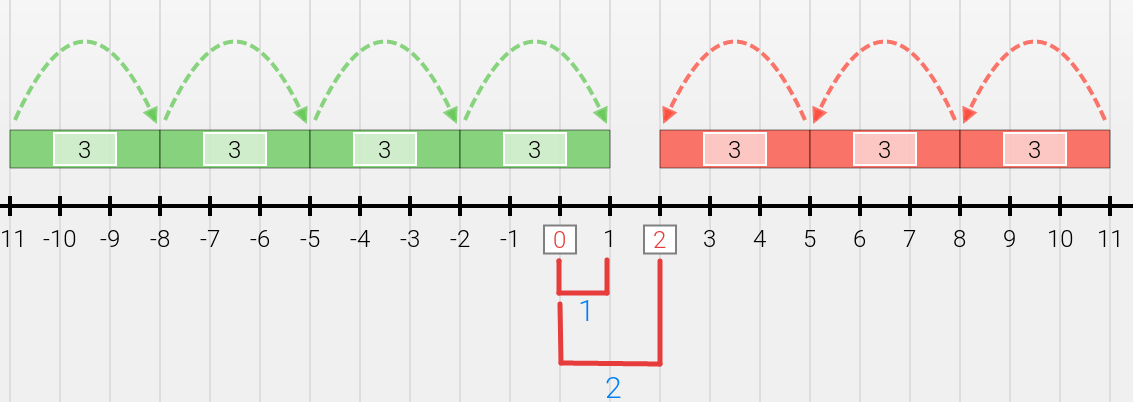
\includegraphics[width=11cm]{mod-num-line.png}
\end{center}
\begin{minipage}[c]{.5\linewidth}

	\par\noindent In the case of \(-11 \mod 3\) we can see that there are 4 skips needed to enter the modulo range. The distance between where the last skip lands and 0 is the modulo. In this case, this distance is 1.

\end{minipage}%%%
\begin{minipage}[c]{.5\linewidth}
	\par\noindent In the case of \(11 \mod 3\) we can see that there are 3 skips needed to enter the modulo range. The distance between where the last skip lands and 0 is the modulo. In this case, this distance is 2.
\end{minipage}
\linebreak
\linebreak
\par\noindent For the operation \(a \mod b\) and if a is negative, then we can calculate the modulo using the following expression:

\begin{flalign}
	a + \lvert \lfloor \frac{a}{b} \rfloor \rvert(b) + b
\end{flalign} 

\subsection{Modular Addition}

\par\noindent The property of modular addition is as follows:

\begin{flalign}
	(a+b)\mod c = (a\mod c + b\mod c )\mod c
\end{flalign} 

\par\noindent This relationship can be derived by using expression (1). As a sidenote, recall that if a is divisible by c, and b is divisible by c, then a+b is divisible by c. We first start by restating a + b:

\begin{flalign*}
a = cq_{1} + r_{1} \therefore a \mod c = r_{1}\\
b = cq_{2} + r_{2} \therefore b \mod c = r_{2}\\
a+b = (cq_{1} + r_{1} + cq_{2} + r_{2}) \\
a+b = c(q_{1} + q_{2}) + r_{1} + r_{2}
\end{flalign*} 

\par\noindent Plugging the above result back into \(a+b) \mod c\) we get:

\begin{flalign*}
	(c(q_{1} + q_{2}) + r_{1} + r_{2}) \mod c
\end{flalign*}

\par\noindent We can apply the following rule to simplify the above expression. If I have an operation \(a \mod b\), then I know that adding a multiple of b (say kb), will result in the same modulo value: \((a + kb) \mod b = a\mod b\). We can now proceed with the following simplification:

\begin{flalign*}
	(c(q_{1} + q_{2}) + r_{1} + r_{2}) \mod c \\
	= (r_{1} + r_{2}) \mod c
\end{flalign*}

\par\noindent On to the right hand side of expression (3), using:

\begin{flalign*}
	a = cq_{1} + r_{1} \therefore a \mod c = r_{1}\\
	b = cq_{2} + r_{2} \therefore b \mod c = r_{2}\\
\end{flalign*}

\par\noindent So the right hand side becomes \( (r_{1} + r_{2}) \mod c\) as well.

\subsection{Modular Multiplication}

\par\noindent The property of modular multiplication is as follows:

\begin{flalign}
	(ab)\mod c= ( (a\mod c) \;\; (b\mod c)) \mod c
\end{flalign}

\par\noindent This can be derived in a way similar like we did with modular addition. The left hand side can be rewritten like so:

\begin{flalign*}
	((cq_{1} + r_{1})(cq_{2} + r_{2})) \mod c \\
	= (  c^{2}   q_{1}  q_{2} + cq_{1}r_{2} + cq_{2}r_{1} + r_{1}r_{2}) \mod c \\
	= (c(cq_{1}q_{2} + q_{1}r_{2} + q_{2}r_{1}) + r_{1}r_{2}) \mod c
\end{flalign*}

\par\noindent Since \(c(cq_{1}q_{2} + q_{1}r_{2} + q_{2}r_{1})\) is a multiple of c, we are left with:

\begin{flalign*}
	(r_{1}r_{2})\mod c
\end{flalign*}

\par\noindent On to the right hand side of expression (4), using:

\begin{flalign*}
	a = cq_{1} + r_{1} \therefore a \mod c = r_{1}\\
	b = cq_{2} + r_{2} \therefore b \mod c = r_{2}\\
\end{flalign*}

\par\noindent We see that the right hand side of expression (4) becomes:

\begin{flalign*}
	(r_{1}r_{2})\mod c
\end{flalign*}

\subsection{Modular Exponentiation}

\par\noindent Modular exponentiation takes the form of evaluation a problem like \(a^{x} \mod b\). The challenge here is that \(a^{x}\) could easily become a very large number, causing errors on calculators. A commonly used technique to overcome this problem is known as "fast modular exponentiation" and it involves restating x using base-2.

\par\noindent Suppose we are trying to evaluate \(7^{15} \mod 17\). The first step is to translate the exponent into base-2. The number 15 thus becomes \( (1111)_{2} \). We can expand this base-2 number with each term representing the binary symbol \{0,1\} times 2 raised to the power of the place value it appears in:

\begin{flalign*}
	15 = (1)(2)^{3} + (1)(2)^{2} + (1)(2)^{1} + (1)(2)^{0}
\end{flalign*}

\par\noindent With this expansion in mind, we can restate the original problem like so:

\begin{flalign*}
	7^{15} \mod 17 \\
	= (7^{(1)2^{3} + (1)2^{2} + (1)2^{1} + (1)2^{0} }) \mod 17 \\
	= (7^{8 + 4 + 2 + 1 }) \mod 17 \\
\end{flalign*}

\par\noindent Finally, we can apply the algebraic rule of exponents along with modular multiplication:

\begin{flalign*}
	(7^{8 + 4 + 2 + 1 }) \mod 17 \\
	= ((7^{8} \mod 17) \;\;\;(7^{4} \mod 17)\;\;\;(7^{2} \mod 17)\;\;\;(7^{1} \mod 17)) \mod 17
\end{flalign*}

\par \noindent We have now broken the problem into individual components, thus making calculations easier and reducing the likelikhood of overflow errors.

\end{document}